\section{Mosaic orientation and axial scattering}
\label{sec:si_mosaic}

Crystallite tilt changes which parts of a reciprocal rod meet the elastic condition. This section defines the angular probability used for that weighting, then separates transverse orientation sensitivity from the radial axial extension discussed in the main text.

\subsection{Wrapped mosaic distribution}
\label{subsec:si_wrapped_mosaic}

The wrapped mosaic profile uses a signed tilt coordinate $\Delta\theta\in(-\pi,\pi]$ relative to the substrate normal. Its periodic continuation identifies angles differing by $2\pi$. The component normalization below is with respect to $d\Delta\theta$. The nonnegative tilt magnitude and the density per solid angle use different measures, as specified below.

The profile is a wrapped Gaussian $G_{\mathrm w}$ plus a wrapped Lorentzian $L_{\mathrm w}$. Their mixture weight is $p_{\mathrm{tail}}$, the Lorentzian half-width is $\Gamma$, and the Gaussian standard deviation is $\sigma$:
\[
  \omega_{\mathrm w}(\Delta\theta;p_{\mathrm{tail}},\Gamma,\sigma)
  =p_{\mathrm{tail}}\,L_{\mathrm w}(\Delta\theta;\Gamma)
  +(1-p_{\mathrm{tail}})\,G_{\mathrm w}(\Delta\theta;\sigma),
  \qquad 0\le p_{\mathrm{tail}} \le 1.
\]
The Lorentzian half-width $\Gamma$ and Gaussian standard deviation $\sigma$ are independent. The wrapped Lorentzian and wrapped Gaussian are
\[
  L_{\mathrm w}(\Delta\theta;\Gamma)=
  \sum_{q=-\infty}^{\infty}\frac{1}{\pi}\frac{\Gamma}{(\Delta\theta+2\pi q)^2+\Gamma^2}
  =\frac{1}{2\pi}\,\frac{\sinh\Gamma}{\cosh\Gamma-\cos\Delta\theta},
\]
\[
  \begin{aligned}
    G_{\mathrm w}(\Delta\theta;\sigma)
    &= \sum_{q=-\infty}^{\infty}\frac{1}{\sqrt{2\pi}\sigma}
       \exp\!\left[-\frac{(\Delta\theta+2\pi q)^2}{2\sigma^2}\right] \\
    &= \frac{1}{2\pi}\!\left[
         1+2\sum_{n=1}^{\infty}e^{-n^2\sigma^2/2}\cos(n\Delta\theta)
       \right].
  \end{aligned}
\]
The integer $q$ labels periodic images and $n$ labels positive Fourier harmonics. Angles in these expressions are in radians. Both components integrate to unity over $(-\pi,\pi]$, so $\omega_{\mathrm w}$ is normalized. The underlying unwrapped Lorentzian FWHM is $2\Gamma$, and the underlying unwrapped Gaussian FWHM is $2\sqrt{2\ln 2}\,\sigma$. The local small-width limit recovers the usual line-shape widths, but the refinement and normalization are defined by the wrapped functions above. The broad functional form is phenomenological. These equations define the two-component model. Establishing its necessity requires comparison with a re-optimized Gaussian-only model.

\subsection{Folded tilt probability and orientation measure}

For the even signed profile above, the probability density of the magnitude $0\leq\alpha\leq\pi$ is
\begin{equation}
p_\alpha(\alpha)=\omega_{\mathrm w}(\alpha)+\omega_{\mathrm w}(-\alpha)
=2\omega_{\mathrm w}(\alpha),\qquad
p_m(\alpha,\beta)=\frac{p_\alpha(\alpha)}{2\pi}.
\label{eq:si_folded_orientation}
\end{equation}
Thus $\int_0^\pi p_\alpha\,d\alpha=1$ and $\int_0^\pi\int_0^{2\pi}p_m\,d\beta\,d\alpha=1$. The angular-line measure uses the flat coordinate element $d\alpha\,d\beta$. When the same normal directions are expressed as a density per solid angle, $d\Omega=\sin\alpha\,d\alpha\,d\beta$, the corresponding density is
\begin{equation}
f_\Omega(\alpha,\beta)=\frac{p_\alpha(\alpha)}{2\pi\sin\alpha},
\qquad 0<\alpha<\pi.
\label{eq:si_orientation_solid_angle}
\end{equation}
The apparent polar singularity is integrable with the solid-angle measure. On a sphere of radius $Q$, the density per surface area is $f_\Omega/Q^2$. A smooth density specified directly per solid angle is a different orientation law. Figure~\ref{fig:si_mosaic_measures} shows these probability conventions.

\begin{figure}[!htbp]
\centering
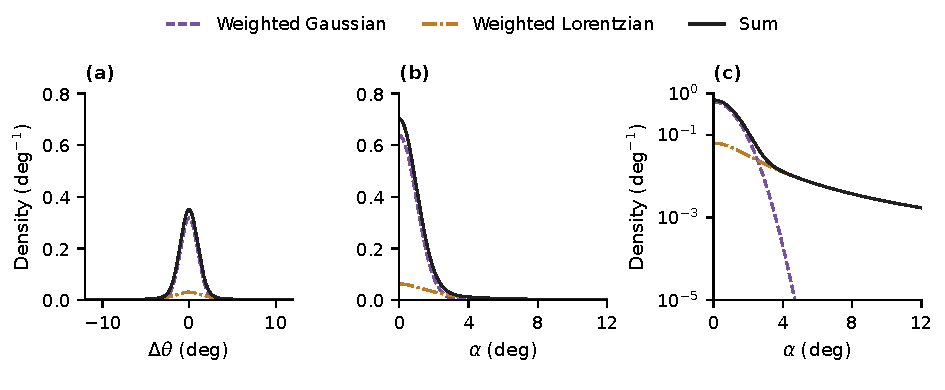
\includegraphics[width=\linewidth]{figures/mosaic_measure_guide.pdf}
\caption{Wrapped angular distributions and their measures. Purple dashed and amber dash-dotted lines show the weighted Gaussian and Lorentzian components, and the black solid line is their sum. (a) Signed density versus $\Delta\theta$. (b) The folded magnitude density on the same linear ordinate scale. (c) The same folded curves on a logarithmic ordinate scale. The parameter values are $\sigma=1^\circ$, $\Gamma=2^\circ$, and $p_{\mathrm{tail}}=0.2$, with azimuth uniform. Ordinates are probability density per degree. Each component is normalized over the complete angular domain before applying its mixture weight, and the displayed windows retain that full-domain normalization. Folding adds the positive and negative signed contributions. The wider component remains visible away from the core.}
\label{fig:si_mosaic_measures}
\end{figure}

The orientation map rotates the entire reciprocal rod, including its basal offset. For the positive-$L$ axial rod, the geometry simplifies to
\begin{equation}
Q_R=|\mathbf c^*|L\sin\alpha,\qquad Q_z=|\mathbf c^*|L\cos\alpha.
\label{eq:si_axial_tilt_geometry}
\end{equation}
Consequently, even an axial point has $L_{\mathrm{proj}}=L\cos\alpha$ after tilt. For an off-axis rod, the rotated basal offset also contributes to projected $Q_z$. Figure~\ref{fig:si_mosaic_results} reserves the material-specific component comparison.


\begin{figure}[!htbp]
  \centering
  \siplaceholder{Material-specific mosaic components}{(a) Bi$_2$Se$_3$ core and tail.\quad (b) Bi$_2$Te$_3$ core and tail.\\Shared linear-core and logarithmic-tail views.}
  \caption{Placeholder for material-specific weighted mosaic components. Direct curves and their matching parameter state are to be inserted with the declared probability measure, full-support normalization, and parameter uncertainties where available.}
  \label{fig:si_mosaic_results}
\end{figure}

\FloatBarrier
\subsection{Controls on the radial axial extension}

The contribution of wavelength spread to an axial feature can be examined
with a mean-wavelength control at fixed remaining inputs. The full detector quantity is
\begin{equation}
  I_{\mathrm{det}}^{\mathrm{full}}(c_D,r_D)=\sum_s w_s I_{\mathrm{det},s}(c_D,r_D;\lambda_s),
  \qquad
  \sum_s w_s=1,
  \label{eq:si_full_spectrum_control}
\end{equation}
Here $I_{\mathrm{det},s}(c_D,r_D;\lambda)$ denotes the detector-coordinate intensity density for the position and direction of state $s$, evaluated at the indicated wavelength $\lambda$. Every state has its own incident wavevector and Ewald intersection. The superscripts $\mathrm{full}$ and $\mathrm{mono}$ identify the full-spectrum and mean-wavelength calculations. The control replaces the distribution by its weighted mean,
\begin{equation}
  I_{\mathrm{det}}^{\mathrm{mono}}(c_D,r_D)=\sum_s w_s I_{\mathrm{det},s}(c_D,r_D;\bar\lambda),
  \qquad
  \bar\lambda=\sum_s w_s\lambda_s,
  \label{eq:si_mean_wavelength_control}
\end{equation}
while holding source positions and directions, their weights, geometry, structural
and mosaic parameters, intensity scale, background treatment, and detector mapping
fixed. Wavelength-dependent scattering factors and optical quantities are
evaluated consistently at the control wavelength.

In the Bi$_2$Se$_3$ and Bi$_2$Te$_3$ model controls, the radial axial extension persisted when wavelength and incident-direction spread were removed. It also persisted when the source was reduced to one monochromatic point ray at the configured mean position and direction. These controls show that the tested model generates the extension even for a monochromatic source.

The model produces continuous finite-stack axial intensity weighted by the orientation distribution near the mean specular direction. In the Bi$_2$Se$_3$ control, changing incidence moved the radial extension from the vicinity of $003$ to $006$ while preserving the structural Bragg positions. Increasing the coherent repeat count reduced the far-tail intensity relative to the integrated Bragg strength. These interventions identify the origin of the extension within the tested model state.

The cause of the measured feature and the relative-order intensity disagreement remain unresolved by these calculations. Radial and transverse profiles provide separate tests of source and orientation effects. Assessing a wavelength effect requires a matched control for the stated geometry and model. Figures~\ref{fig:si_axial_controls} and~\ref{fig:si_mosaic_ablation} reserve the direct control calculations and the separate test of component necessity.


\begin{figure}[!htbp]
  \centering
  \siplaceholder{Radial-extension controls}{(a) Full source and monochromatic point ray.\\(b) Incidence transfer from the vicinity of 003 to 006.\\(c) Coherent-repeat control at fixed remaining inputs.}
  \caption{Placeholder for direct model controls on the radial axial extension. The intended panels compare identical detector regions and declared common scales while varying source spread, incidence, or coherent repeat count separately. The controls test the retained model mechanism.}
  \label{fig:si_axial_controls}
\end{figure}


\begin{figure}[!htbp]
  \centering
  \siplaceholder{Controlled mosaic comparison}{Two-component model, same-state no-tail control, and reoptimized Gaussian-only model.\\Matched profiles, residuals, and uncertainty across incidence angles.}
  \caption{Placeholder for the controlled test of a broad mosaic component. A comparison requires direct calculated arrays, identical measured regions, declared nuisance parameters, and a common residual criterion.}
  \label{fig:si_mosaic_ablation}
\end{figure}
